\documentclass[aspectratio=169]{beamer}

% ── Theme ─────────────────────────────────────────────────────────────────────
\usetheme{Madrid}
\usecolortheme{whale}
\setbeamertemplate{navigation symbols}{}
\setbeamertemplate{footline}[frame number]

% ── Packages ──────────────────────────────────────────────────────────────────
\usepackage{amsmath,amssymb}
\usepackage{graphicx}
\usepackage{booktabs}
\usepackage{multirow}
\usepackage{tikz}
\usetikzlibrary{arrows.meta,positioning,shapes.geometric,fit,calc}
\usepackage{pgfplots}
\pgfplotsset{compat=1.18}
\usepackage{subcaption}
\usepackage{xcolor}

% ── Colors ────────────────────────────────────────────────────────────────────
\definecolor{pos}{RGB}{34,139,34}
\definecolor{neg}{RGB}{180,30,30}
\definecolor{neu}{RGB}{100,100,180}

% ── Macros ────────────────────────────────────────────────────────────────────
\newcommand{\pp}{\,pp}
\newcommand{\cifar}{CIFAR-10}
\newcommand{\good}[1]{{\color{pos}\textbf{#1}}}
\newcommand{\bad}[1]{{\color{neg}\textbf{#1}}}

% ── Title ─────────────────────────────────────────────────────────────────────
\title[CNN Tricks $\to$ Transformers?]{Do CNN Speed-Up Tricks Transfer\\to Transformers?}
\subtitle{COMP-4471: Deep Learning in Computer Vision}
\author{Siwei LIU \and Xingjian ZHANG \and Liwei LI}
\institute{The Hong Kong University of Science and Technology}
\date{}

% ══════════════════════════════════════════════════════════════════════════════
\begin{document}

% ── Slide 1: Title ────────────────────────────────────────────────────────────
\begin{frame}
\titlepage{}
\end{frame}

% ── Slide 2: Motivation & Gap ─────────────────────────────────────────────────
\begin{frame}{Motivation \& Research Gap}
\begin{columns}
\begin{column}{0.52\textwidth}
    \textbf{Garg et al.\ (2024)} — 4 tricks for fast CNN training on \cifar{}:
    \begin{enumerate}
        \item Frozen patch-whitening init
        \item Dirac (identity) init
        \item ScaleBias + Lookahead
        \item Alternating flip
    \end{enumerate}
    \Large\centering $\Rightarrow$ \textbf{94\% in 3.29 s}
\end{column}
\begin{column}{0.44\textwidth}
    \centering
    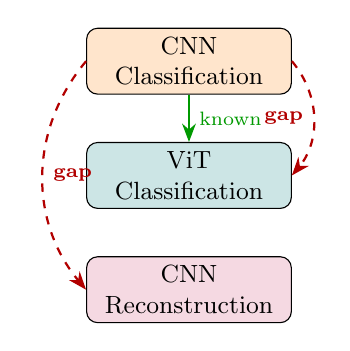
\begin{tikzpicture}[node distance=0.6cm,
        box/.style={draw,rounded corners,fill=blue!10,minimum width=2.6cm,
                    minimum height=0.65cm,font=\small,align=center}]
        \node[box,fill=orange!20] (cnn) {CNN\\Classification};
        \node[box, below=of cnn, fill=teal!20] (vit) {ViT\\Classification};
        \node[box, below=of vit, fill=purple!15] (rec) {CNN\\Reconstruction};
        \draw[-{Stealth},thick,green!60!black] (cnn) -- node[right,font=\scriptsize]{known} (vit);
        \draw[-{Stealth},thick,red!70!black,dashed] (cnn.east)
            to[bend left=40] node[left,font=\scriptsize,red!70!black]{\textbf{gap}} (vit.east);
        \draw[-{Stealth},thick,red!70!black,dashed] (cnn.west)
            to[bend right=40] node[right,font=\scriptsize,red!70!black]{\textbf{gap}} (rec.west);
    \end{tikzpicture}
    \vspace{1em}
    {\small Do tricks transfer across architectures \& tasks?}
\end{column}
\end{columns}
\end{frame}

% ── Slide 3: Model & Two Recipes ──────────────────────────────────────────────
\begin{frame}{Our ViT \& Two Training Recipes}
\begin{columns}
\begin{column}{0.44\textwidth}
    \centering
    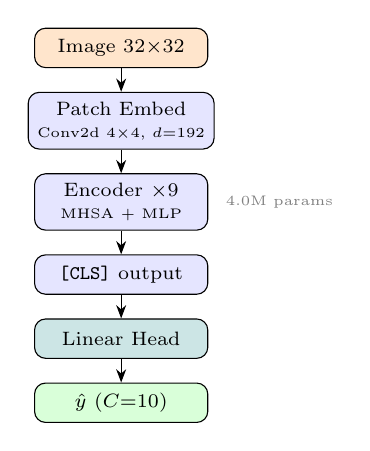
\begin{tikzpicture}[node distance=0.3cm,
        b/.style={draw,rounded corners,fill=blue!10,
                  minimum width=2.2cm,minimum height=0.5cm,
                  font=\scriptsize,align=center}]
        \node[b,fill=orange!20] (img) {Image $32{\times}32$};
        \node[b,below=of img] (pe) {Patch Embed\\{\tiny Conv2d $4{\times}4$, $d{=}192$}};
        \node[b,below=of pe] (enc) {Encoder $\times 9$\\{\tiny MHSA + MLP}};
        \node[b,below=of enc] (cls) {\texttt{[CLS]} output};
        \node[b,below=of cls,fill=teal!20] (head) {Linear Head};
        \node[b,below=of head,fill=green!15] (pred) {$\hat{y}\ (C{=}10)$};
        \foreach \a/\b in {img/pe,pe/enc,enc/cls,cls/head,head/pred}
            \draw[-{Stealth}] (\a)--(\b);
        \node[right=0.1cm of enc,font=\tiny,gray] {4.0M params};
    \end{tikzpicture}
\end{column}
\begin{column}{0.52\textwidth}
    \small
    \begin{tabular}{lcc}
        \toprule
        & \textbf{Weak} & \textbf{Strong} \\
        \midrule
        Epochs     & 100  & 300 \\
        Peak LR    & $3\times10^{-4}$ & $1\times10^{-3}$ \\
        Schedule   & OneCycleLR & Cosine \\
        DropPath   & --- & 0.1 \\
        RandAugment & --- & \checkmark{} \\
        Mixup/CutMix & --- & \checkmark{} \\
        \midrule
        \textbf{Baseline} & \textbf{61.7\%} & \textbf{81.4\%} \\
        \bottomrule
    \end{tabular}
\end{column}
\end{columns}
\end{frame}

% ── Slide 4: The Four Tricks ──────────────────────────────────────────────────
\begin{frame}{The Four Tricks — Adapted for ViT}
\begin{columns}
\begin{column}{0.48\textwidth}
    \textbf{1. Frozen Patch-Whitening}
    \[
        W_k = \frac{\mathbf{v}_k}{\sqrt{\lambda_k + \varepsilon}},\quad
        \texttt{requires\_grad=False}
    \]
    \vspace{0.4em}
    \textbf{2. Dirac / Soft Dirac Init}
    \[
        \mathbf{W}_{QKV} = \mathbf{I}_D, \qquad
        \mathbf{W} \leftarrow \alpha\mathbf{I} + (1{-}\alpha)\mathbf{W}_\text{rand}
    \]
\end{column}
\begin{column}{0.48\textwidth}
    \textbf{3. ScaleBias + Lookahead}
    \[
        y_i = s_i x_i + b_i,\quad
        \phi \leftarrow \phi + \alpha(\theta{-}\phi)
    \]
    \vspace{0.4em}
    \textbf{4. Alternating Flip}
    \begin{center}
        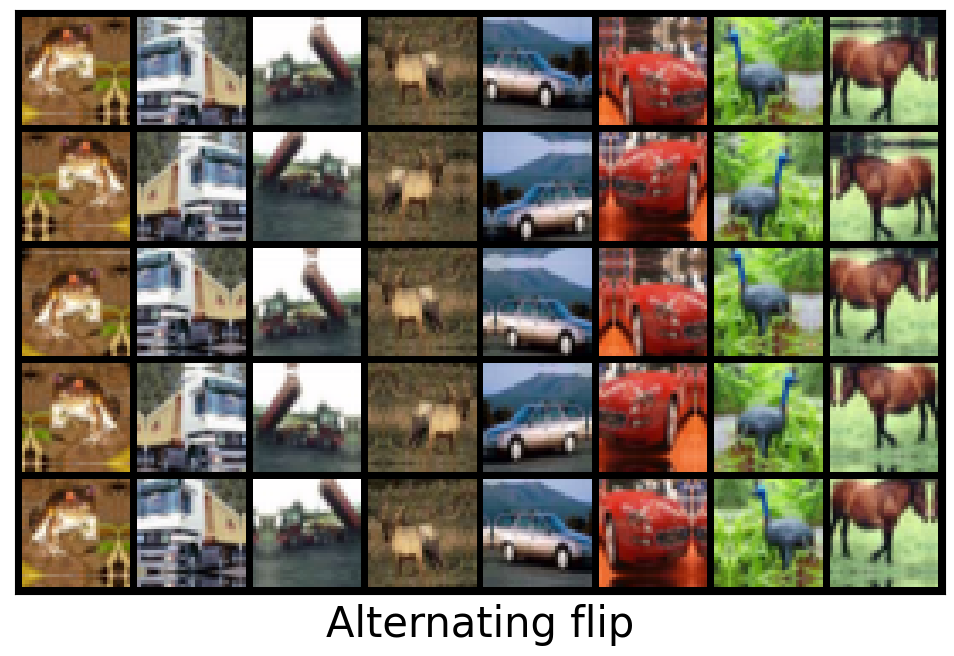
\includegraphics[width=0.85\linewidth]{figures/alternating_flip.png}
    \end{center}
    {\scriptsize Every odd-indexed sample is always flipped}
\end{column}
\end{columns}
\end{frame}

% ── Slide 5: Classification Results ──────────────────────────────────────────
\begin{frame}{Classification Results: Trick $\times$ Recipe Interaction}
\centering
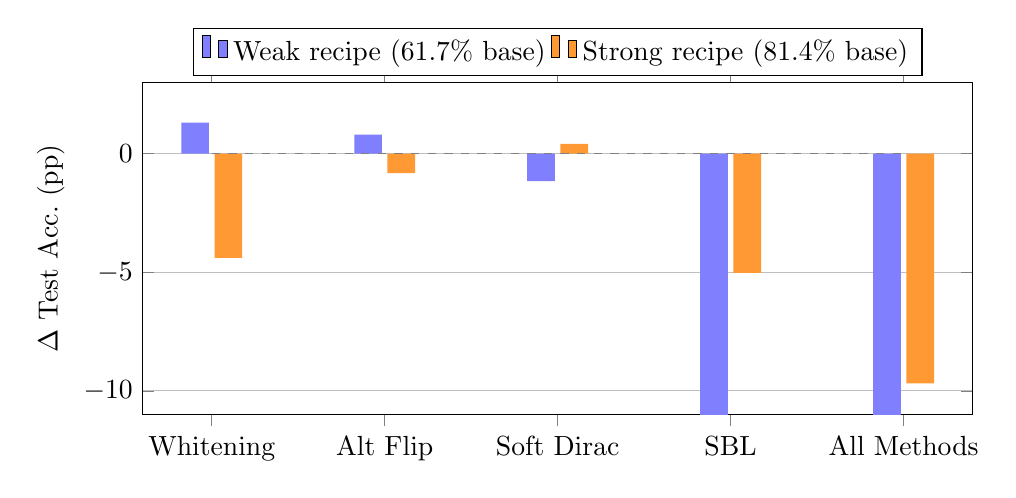
\begin{tikzpicture}
\begin{axis}[
    ybar, bar width=10pt,
    width=\textwidth, height=5.8cm,
    symbolic x coords={Whitening,Alt Flip,Soft Dirac,SBL,All Methods},
    xtick=data,
    xlabel={},
    ylabel={$\Delta$ Test Acc.\ (pp)},
    ymin=-11, ymax=3,
    ymajorgrids=true,
    legend style={at={(0.5,1.02)},anchor=south,legend columns=2},
    every axis plot/.append style={draw=none},
]
% Weak recipe bars
\addplot[fill=blue!50] coordinates {
    (Whitening,    1.31)
    (Alt Flip,     0.80)
    (Soft Dirac,  -1.16)
    (SBL,        -15.97)
    (All Methods,-23.63)
};
% Strong recipe bars
\addplot[fill=orange!80] coordinates {
    (Whitening,   -4.39)
    (Alt Flip,    -0.82)
    (Soft Dirac,   0.41)
    (SBL,         -5.03)
    (All Methods, -9.68)
};
\legend{Weak recipe (61.7\% base), Strong recipe (81.4\% base)}
\draw[dashed,gray] (axis cs:Whitening,0) -- (axis cs:All Methods,0);
\end{axis}
\end{tikzpicture}

\vspace{-0.5em}
{\small \bad{Whitening flips from $+1.3$\pp{} to $-4.4$\pp{}}
\quad\good{Soft Dirac: only net-positive under strong recipe ($+0.4$\pp{})}}
\end{frame}

% ── Slide 6: Whitening Conflict ───────────────────────────────────────────────
\begin{frame}{Why Does Whitening Reverse? The Frozen-Embedding Conflict}
\begin{columns}
\begin{column}{0.44\textwidth}
    \centering
    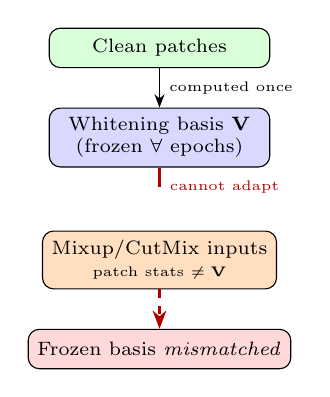
\begin{tikzpicture}[node distance=0.5cm,
        b/.style={draw,rounded corners,minimum width=2.8cm,
                  minimum height=0.5cm,font=\scriptsize,align=center}]
        \node[b,fill=green!15] (clean) {Clean patches};
        \node[b,below=of clean,fill=blue!15] (basis) {Whitening basis $\mathbf{V}$\\(frozen $\forall$ epochs)};
        \node[b,below=0.8cm of basis,fill=orange!25] (mix) {Mixup/CutMix inputs\\{\tiny patch stats $\neq \mathbf{V}$}};
        \node[b,below=of mix,fill=red!15] (bad) {Frozen basis \emph{mismatched}};
        \draw[-{Stealth}] (clean)--(basis)
            node[midway,right,font=\tiny]{computed once};
        \draw[-{Stealth},dashed,red!70!black,thick] (mix)--(bad);
        \draw[red!70!black,thick] (basis.south) -- ++(0,-0.25)
            node[right,font=\tiny,red!70!black] {cannot adapt};
    \end{tikzpicture}
\end{column}
\begin{column}{0.52\textwidth}
    \centering
    \textbf{CNN Reconstruction (no Mixup): conflict absent}\\[0.3em]
    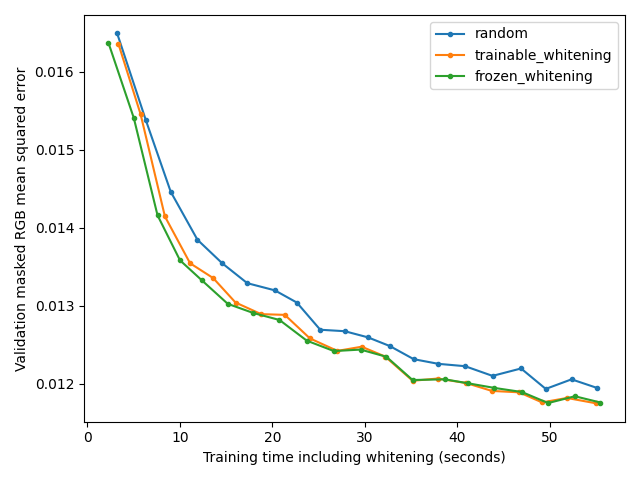
\includegraphics[width=\linewidth]{figures/cnn_reconstruction.png}\\[0.2em]
    {\small Frozen $\approx$ Trainable whitening\\
    Freezing \emph{itself} is \textbf{not} the problem}
\end{column}
\end{columns}
\end{frame}

% ── Slide 7: Reconstruction Results ──────────────────────────────────────────
\begin{frame}{CNN Reconstruction: All Tricks Help}
\begin{columns}
\begin{column}{0.52\textwidth}
    \centering
    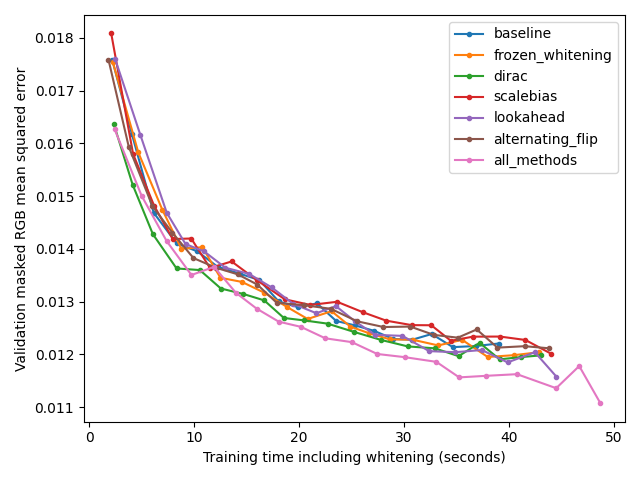
\includegraphics[width=\linewidth]{figures/cnn_reconstruction_full.png}
\end{column}
\begin{column}{0.44\textwidth}
    \small
    \begin{tabular}{lc}
        \toprule
        Variant          & $\Delta$ MSE \\
        \midrule
        Baseline         & ---          \\
        Whitening        & \good{$-1.4\%$} \\
        Alt Flip         & \good{$-0.8\%$} \\
        ScaleBias        & \good{$-1.6\%$} \\
        Dirac            & \good{$-1.8\%$} \\
        \textbf{Lookahead} & \good{$\mathbf{-5.1\%}$} \\
        \midrule
        \textbf{All methods} & \good{$\mathbf{-9.3\%}$} \\
        \bottomrule
    \end{tabular}
    \vspace{0.5em}

    \textbf{Key:} Lookahead works here\\
    (flat Adam LR = no schedule conflict)
\end{column}
\end{columns}
\end{frame}

% ── Slide 8: Unified Framework ────────────────────────────────────────────────
\begin{frame}{A Two-Axis Compatibility Framework}
\centering
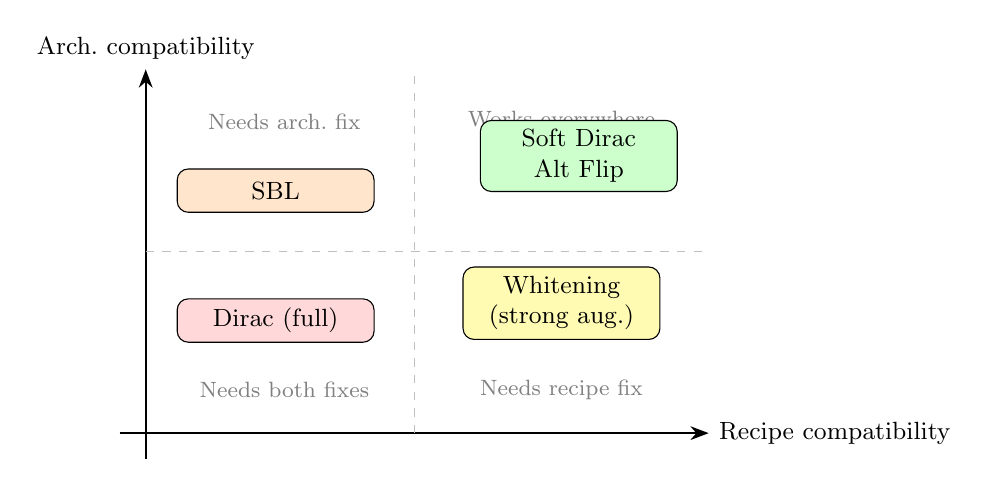
\begin{tikzpicture}[scale=1.1,
    trick/.style={draw,rounded corners,minimum width=2.5cm,
                  minimum height=0.55cm,font=\small,align=center}]

    % Axes
    \draw[-{Stealth},thick] (-0.3,0) -- (6.5,0)
        node[right,font=\small] {Recipe compatibility};
    \draw[-{Stealth},thick] (0,-0.3) -- (0,4.2)
        node[above,font=\small] {Arch.\ compatibility};

    % Quadrant labels
    \node[gray,font=\footnotesize] at (1.6,3.6) {Needs arch.\ fix};
    \node[gray,font=\footnotesize] at (4.8,3.6) {Works everywhere};
    \node[gray,font=\footnotesize] at (1.6,0.5) {Needs both fixes};
    \node[gray,font=\footnotesize] at (4.8,0.5) {Needs recipe fix};

    % Grid
    \draw[dashed,gray!50] (3.1,0) -- (3.1,4.2);
    \draw[dashed,gray!50] (0,2.1) -- (6.5,2.1);

    % Tricks
    \node[trick,fill=red!15] at (1.5,1.3) {Dirac (full)};
    \node[trick,fill=orange!20] at (1.5,2.8) {SBL};
    \node[trick,fill=yellow!30] at (4.8,1.5) {Whitening\\(strong aug.)};
    \node[trick,fill=green!20] at (5.0,3.2) {Soft Dirac\\Alt Flip};

\end{tikzpicture}
\end{frame}

% ── Slide 9: Conclusion ───────────────────────────────────────────────────────
\begin{frame}{Conclusion \& Future Work}
\begin{columns}
\begin{column}{0.52\textwidth}
    \textbf{Key finding}
    \[
        \text{Transferability} = \text{trick} \times \text{recipe}
    \]
    \vspace{0.3em}
    \begin{itemize}
        \item Whitening: good with simple aug.,\\
              bad with Mixup/CutMix
        \item Dirac: bad in attn., good in CNN conv.
        \item Lookahead: bad with decaying LR,\\
              good with flat LR
        \item \good{Soft Dirac only net-positive\\in strong ViT recipe}
        \item \good{All tricks help in reconstruction}
    \end{itemize}
\end{column}
\begin{column}{0.44\textwidth}
    \textbf{Future work}
    \vspace{0.5em}
    \begin{enumerate}
        \item \textbf{Learnable whitening}\\
              {\small let embedding adapt to Mixup inputs}
        \item \textbf{Decayed soft Dirac}\\
              {\small anneal $\alpha \to 0$ over first 20 epochs}
        \item \textbf{Lookahead + flat LR}\\
              {\small decouple from schedule}
    \end{enumerate}
    \vspace{0.5em}
    {\small Test each trick under the \emph{full}\\
    target recipe before adopting it.}
\end{column}
\end{columns}
\end{frame}

\end{document}
